\documentclass[10pt]{article}

\usepackage[utf8]{inputenc}

\usepackage{geometry}
\geometry{a4paper, margin=0.5in}

\usepackage{amsmath}
\usepackage{amssymb}

\usepackage{hyperref}

% Adding paragraphs as proper titles
\usepackage{titlesec}
\setcounter{secnumdepth}{5}

\usepackage[
    backend=biber,
    style=numeric,
    url=true
]{biblatex}
\addbibresource{../references/references.bib}

\usepackage{graphicx}
\graphicspath{{./img/}}

\begin{document}

\title{Comparing Correlation Functions and Exploring Efficiency and Identifiability Issues for the Gaussian Process}
\author{
    Ivor Walker \\
    Supervised by Dr Michail Papathomas \\
}
\date{ }
\maketitle



\section*{Abstract}

% This project concerns the Gaussian process. The student will be required to understand the Gaussian process model and the different applications where it is employed, in relation to statistical modelling and machine learning, by reading relevant textbooks and publications. Then, using simulated and real data, different correlation functions will be explored and compared. Other aspects of the Gaussian process (GP) will be explored. Computational efficiency, for instance, as using the GP typically requires the inversion of large matrices, or identifiability issues when the GP is used to model the residuals after a linear model is fitted.

\newpage
\tableofcontents
\newpage



\section{Introduction}



\section{Defining the Gaussian Process}



\subsection{Weight-space view \cite{gp-ml}}

\subsubsection{Standard linear model}
The standard linear model neatly summarises how all data ever produced in the universe has been generated. It summises that we have some data-generating function $f(.)$ that combines training data $X$ and parameters of the model $W$ to produce an output $y$:
\begin{equation} \label{eq:linear_model}
    \begin{aligned}
        y = f(X) + \epsilon \\
        f(X) = X^T W \\
    \end{aligned}
\end{equation}

$y$ is rarely a perfect observation of $f(X)$, e.g. because of measurement error, so we add some noise $\epsilon$. The standard linear model assumes that our noise term can be drawn from a Gaussian distribution $\epsilon \sim N(0, \sigma_n^2I)$. We add a covariance matrix $I$ to describe how the noise for one observation is related to the noise of another observation, e.g. how a burst of noise affects some observations but not others. 

We can combine our expressions and assumptions for $f(X)$ and $\epsilon$ to produce the distribution of errors, or the distribution from which $y$ is drawn from after knowing perfectly $X$ and $W$:
\begin{equation*}
    p(y|X,W) = \mathcal{N}(y | X^TW, \sigma^2_nI)
\end{equation*}

Our first task is to find $W$ as we typically do not know it in advance. Frequentist statistics focuses on arriving at a single estimate of $W$ ($\hat{W}$) via MLE (maximum likelihood estimation). $p(y|X,W)$ is at its highest density around our error $y | X^TW$ and we assumed our error zero, so we can use optimisation methods to find $\hat{W}$ to find the highest density of the distribution $N(0, \sigma^2_nI)$, which is the same as minimising the squared error $||y - X^TW||^2$. However, a single $\hat{W}$ does not tell us how confident we are in our estimate, or how much uncertainty there is in the model. 

Bayesian statistics addresses this by treating $W$ as a random variable. We start with a "prior" distribution of $W$, which the Bayesian linear model assumes:
\begin{equation} \label{eq:prior_distribution}
    p(W) \sim N(0, \Sigma_p)
\end{equation}
Then, we observe the data and update our beliefs about the weights using Bayes' theorem to produce a "posterior" distribution $p(W|X,y)$.

\begin{equation*}
    p(W|X,y) = \frac{p(y|X,W)p(W)}{p(y|X)}
\end{equation*}

$p(y|X,W)$ is the density of the residuals after applying our priors $p(W)$ to the data $X,W$ under our assumed noise model $\epsilon$, $p(W)$ is the prior distribution of the weights, and $p(y|X)$ is the marginal likelihood, or how likely the data is given the model.   


\subsubsection{Posterior distribution}
\paragraph{Deriving our posterior}
Because we need to understand how our posterior varies with our weights only, we can ignore terms that do not vary with $W$ such as our marginal likelihood by absorbing it into the proportionality constant. 
\begin{equation} \label{eq:posterior}
    p(W|X, y) \propto p(y|X,W)p(W)
\end{equation}

Starting with $p(Y|X,W)$, we can write it as the distribution of errors for each data point $i$:
\begin{equation*}
    p(y|X,W) = \prod_{i=1}^N \mathcal{N}(y_i|X^TW, \sigma^2_n)
\end{equation*}

We can find $p(y|X,W)$ by multiplying the Gaussian density $-\frac{1}{2\sigma^2_n}$ and the squared errors from our model $||y -X^TW||^2$ to get a final likelihood:
\begin{equation} \label{eq:likelihood}
    p(y|X,W) = exp\left(-\frac{1}{2\sigma^2_n}||y -X^TW||^2\right)
\end{equation}

Then, we can rewrite our $p(W)$ as its density function:
 \begin{equation*}
     p(W) = \frac{1}{[\sqrt{\sigma_p}]\sqrt{2\pi}} exp\left(-\frac{1}{2}\frac{([W]-[0])}{[\Sigma_p]}\right)
\end{equation*}

The first term can be absorbed into the proportionality constant, so rewriting the second term as negative exponential:
\begin{equation} \label{eq:prior_pdf}
    p(W) \propto exp\left(-\frac{1}{2}W^T\Sigma_p^{-1}W\right)
\end{equation}

Putting both expressions for \ref{eq:likelihood} and \ref{eq:prior_pdf} back into the posterior: 
\begin{equation*}
    p(W|X,y) \propto exp\left(-\frac{1}{2\sigma^2_n}||y -X^TW||^2\right)exp\left(-\frac{1}{2}W^T\Sigma_p^{-1}W\right)
\end{equation*}

To simplify, first we can expand $||y - X^TW||^2$ to $y^Ty - 2y^TXW + W^TX^TXW$, and insert this expanded expression:
\begin{equation*}
    p(W|X,y) \propto exp\left(-\frac{1}{2\sigma^2_n}(y^Ty - 2y^TXW + W^TX^TXW)\right)exp\left(-\frac{1}{2}W^T\Sigma_p^{-1}W\right)
\end{equation*}

Then, we put both exponentials together by adding their powers:
\begin{equation*}
    p(W|X,y) \propto exp\left(\frac{1}{\sigma^2_n}(y^Ty - 2y^TXW + W^TX^TXW) + \left(-\frac{1}{2}W^T\Sigma_p^{-1}W\right)\right)
\end{equation*}

We can rearrange the inside term to be a quadratic, linear and constant term in $W$:
\begin{equation*}
    p(W|X,y) \propto exp\left(\frac{1}{2}W^T\left(\frac{1}{\sigma^2_n}X^TX + \Sigma_p^{-1}\right)W - \left(\frac{1}{\sigma^2_n}y^TX\right)W + \frac{1}{2}y^Ty\right)
\end{equation*}

We can ignore the constant final term, and introduce these terms:
\begin{equation} \label{eq:A_b}
    \begin{aligned}
        A = \Sigma_p^{-1} + \frac{1}{\sigma^2_n}X^TX \\
        b = \frac{1}{\sigma^2_n}y^TX
    \end{aligned}
\end{equation}

To get our final posterior's PDF:
\begin{equation*}
    p(W|X,y) \propto exp\left(-\frac{1}{2}W^TAW + b^TW\right)
\end{equation*}

\paragraph{Deriving the properties of the posterior by completing the square}
Now we have a simplified form of the posterior's PDF, we need to get it into a Gaussian form to recover the properties of the posterior distribution.

Firstly, we can bring all terms inside the exponential to a single term:
\begin{equation*}
    -\frac{1}{2}W^TAW + b^TW = \frac{1}{2}\left(-W^TAW + 2b^TW\right)
\end{equation*}

We can "complete the square" on this term $W^TAW - 2b^TW$ to rewrite it in a form that is easier to interpret:
\begin{equation*}
    W^TAW - 2b^TW = (W - A^{-1}b)^TA(W - A^{-1}b) - b^TA^{-1}b
\end{equation*}

Substituting this back into our posterior density:
\begin{equation*}
    p(W|X,y) \propto exp\left(-\frac{1}{2}\left((W - A^{-1}b)^TA(W - A^{-1}b) - b^TA^{-1}b\right)\right)
\end{equation*}

If we look at our Gaussian probability density function (PDF): 
\begin{equation} \label{eq:gaussian_pdf}
    N(W | \mu, \Sigma) = \frac{1}{\sqrt{(2\pi)^d |\Sigma|}} exp\left(-\frac{1}{2}(W - \mu)^T\Sigma^{-1}(W - \mu)\right)
\end{equation}

We can see that our expression lines up with the RHS Gaussian "kernel" term $exp\left(-\frac{1}{2}(W - \mu)^T\Sigma^{-1}(W - \mu)\right)$, where $\mu = A^{-1}b$ and $\Sigma^{-1} = A$ thus $\Sigma = A^{-1}$
So we can write our posterior density in Gaussian form
\begin{equation} \label{eq:posterior_gaussian}
    p(W|X,y) \sim N(A^{-1}b, A^{-1})
\end{equation}

Finally, we lack an expression for $\Sigma_p$ in $A$. The standard linear model assumes independence of noise, so our weight variance $\Sigma_p$ under the Bayesian linear model is "isotropic", meaning it is the same in all directions.
\begin{equation*}
    \Sigma_p = \tau^2 I
\end{equation*}
Because we assume independence, $I$ is an "identity matrix where each diagonal element is 1 and all off-diagonal elements are 0. $\tau^2$ is a scalar variance term, chosen as a prior.

We can substitute our isotropic prior $\Sigma_p$ into $A$:
\begin{equation*}
    A = \Sigma_p^{-1} + \frac{1}{\sigma^2_n}X^TX = \left[{\tau^2}I\right]^{-1} + \frac{1}{\sigma^2_n}X^TX =  \frac{1}{\tau^2}I + \frac{1}{\sigma^2_n}X^TX
\end{equation*}

Simplifying this gives us our final expression for $A$:
\begin{equation} \label{eq:A_isotropic}
A = \frac{1}{\sigma_n^2}\left(X^TX + \frac{\sigma_n^2}{\tau^2}I\right)
\end{equation}

\paragraph{Gaussian posteriors and ridge regression}
For Gaussian posteriors, our mean $A^{-1}b$ is also its mode, called the maximum a posteriori (MAP) estimate of W. This is due to symmetries in linear model and posterior and is not the case in general. Our MAP point is equivelant to our frequentist $\hat{W}$. 

We can substitute our full expressions for $A$ \ref{eq:A_isotropic} and $b$ \ref{eq:A_b} into our MAP estimation to understand how our expressions relate to frequentist approaches:
\begin{equation*} 
    W_{\text{MAP}} = A^{-1}b = \left[\frac{1}{\sigma_n^2}(X^TX + \frac{\sigma_n^2}{\tau^2}I\right]^{-1} \cdot \left[\frac{1}{\sigma_n^2}y^TX\right] \\
\end{equation*}

Inverting LHS term of $A$:
\begin{equation*}
    A^{-1} = \frac{\sigma_n^2}{X^TX + \frac{\sigma_n^2}{\tau^2}I} = \sigma_n^2\left(X^TX + \frac{\sigma_n^2}{\tau^2}I\right)^{-1}
\end{equation*}

Substituting this back into $W_\text{MAP}$ cancels out the $\sigma_n^2$ term in A with the $\frac{1}{\sigma_n^2}$ term in B:
\begin{equation*}
    W_{\text{MAP}} = \sigma_n^2\left(X^TX + \frac{\sigma_n^2}{\tau^2}I\right)^{-1} \cdot \frac{1}{\sigma_n^2}y^TX = \left(X^TX + \frac{\sigma_n^2}{\tau^2}I\right)^{-1} \cdot y^TX
\end{equation*}

The solution to frequentist ridge regression is very similar
\begin{equation*}
    W_{\text{ridge}} = \left(X^TX + \lambda I\right)^{-1}X^Ty
\end{equation*}

In ridge regression, $\lambda$ is a regularisation parameter that controls the amount of shrinkage which is usually selected to maximise likelihood/minimise error. Therefore, our MAP estimation in Bayesian linear regression with isotropic priors is equivalent to ridge regression with $\lambda = \frac{\sigma_n^2}{\tau^2}$. 

The more we trust our prior, the higher our $\lambda$ and the more we shrink our weights towards zero. A lower $\tau$ means we are more confident in $p(W)$ and have better priors, whereas a higher $\sigma_n$ means lower confidence in $p(y|X,W)$ and worse weights.
        
\subsubsection{Predictive distribution}
\paragraph{Deriving the predictive distribution}
Our second task is to make predictions $y_*$ using new input data $X_*$ and our previously learned weights $W$. Frequentist methods simply multiply $\hat{W}$ by $X_*$, but this does not properly propagate the uncertainty in $W$. In this Bayesian framework, we form a "predictive distribution" which we sample from to get our noise-free function evaluations $f(X_*)$ (denoted $f_*$) and add $\epsilon$ to get our noisy predictions $y_*$.

\begin{equation*}
    p(f_*|X_*,X,y) = \int p(f_*|X_*,W) \cdot p(W | X,y)dW
\end{equation*}
$p(f_*|X_*,W)$ is what we think the function looks like after producing a prediction using $X_*$ and perfect knowledge of $W$. $p(W|X,y)$ is our familiar \ref{eq:posterior_gaussian} posterior distribution of weights. $p(f_*|X_*,W) \cdot p(W|X,y)$ is the joint distribution of our predictions and our posterior weights, which gets us the conditional distribution $p(f_*,W|X_*,X,y)$ by definition of conditional probability. Because $p(f_*,W|X_*,X,y)$ relies on our perfect knowledge of $W$, which we lack, we integrate over all possible $W$ to get the final predictive distribution $p(f_*|X_*,X,y)$
    
 $p(f_*|X_*,W)$ is our errors, which we assume to be distributed normally and independently with our $I$ identity matrix:
\begin{equation*}
    p(f_* | X_*, W) = \mathcal{N}(f_* | W^TX_*, \sigma^2_nI)
\end{equation*}

Substituting into \ref{eq:gaussian_pdf} and absorbing the LHS term into the proportionality constant:
\begin{equation*}
    p(f_*|X_*,w) \propto exp\left(-\frac{1}{2}\frac{1}{\sigma^2_n}(f_* - W^TX_*)^2\right)
\end{equation*}

Multiplying $P(f_*|X_*,W)$ and $p(W|X,y)$ to get our conditional $p(f_*, W|X_*,X,y)$, and add the exponents: 
\begin{equation*}
    p(f_*,W|X_*,X,y) \propto exp\left(\frac{1}{2}(-W^TAW + 2b^TW) + \left(-\frac{1}{2}\frac{1}{\sigma^2_n}(f_* - W^TX_*)^2\right)\right)
\end{equation*}

We can further combine these with a single factor of $\frac{1}{2}$:
\begin{equation*}
    p(f_*,W|X_*,X,y) \propto exp\left(-\frac{1}{2}\left(W^TAW - 2b^TW + \frac{1}{\sigma^2_n}(f_* - W^TX_*)^2\right)\right)
\end{equation*}

Expanding the squared term:
\begin{equation*}
    p(f_*,W|X_*,X,y) \propto exp\left(-\frac{1}{2}\left(W^TAW - 2b^TW + \frac{1}{\sigma^2_n}(f_*^2 - 2f_*W^TX_* + W^TX_*X_*^TX_*)\right)\right)
\end{equation*}

Similar to our posterior, we can rearrange this to be a quadratic, linear and constant term in $W$:
\begin{equation*}
    p(f_*,W|X_*,X,y) \propto exp\left(-\frac{1}{2}\left(W^T\left(A + \frac{1}{\sigma^2_n}X_*X_*^T\right)W - 2\left(b + \frac{1}{\sigma^2_n}f_*X_*\right)^TW + \frac{1}{\sigma_n^2}f_*^2\right)\right)
\end{equation*}

We can define:
\begin{equation*}
    \begin{aligned}
        A_* = A + \frac{1}{\sigma^2_n}X_*X_*^T \\
        b_* = b + \frac{1}{\sigma^2_n}f_*X_*
    \end{aligned}
\end{equation*}

And substitute these into our expression to get our final conditional distribution of $f_*,W$:
\begin{equation*}
    p(f_*,W|X_*,X,y) \propto exp\left(-\frac{1}{2}\left(W^TA_*W - 2b_*^TW + \frac{1}{\sigma_n^2}f_*^2\right)\right)
\end{equation*}

Lastly, we have to integrate this wrt $W$ to get our predictive distribution $p(f_*|X_*,X,y)$:
\begin{equation*}
    p(f_*|X_*,X,y) = \int p(f_*,W|X_*,X,y)dW \propto \int exp\left(-\frac{1}{2}\left(W^TA_*W - 2b_*^TW + \frac{1}{\sigma_n^2}f_*^2\right)\right)dW
\end{equation*}

We can factor out the $\frac{1}{\sigma_n^2}f_*^2$ term from the integral, as it does not depend on $W$ (since $\int exp(X) dX = exp(X)$):
\begin{equation*}
    = exp\left(-\frac{1}{2}\frac{1}{\sigma_n^2}f_*^2\right) \times \int exp\left(-\frac{1}{2}\left(W^TA_*W - 2b_*^TW\right)\right) dW
\end{equation*}

The RHS term is a multivariate Gaussian integral which evaluates to:
\begin{equation*}
    \int exp\left(-\frac{1}{2} \left( W^TA_*W - 2b_*^TW \right) \right) dW = \frac{(2\pi)^{D/2}} {\sqrt{|A_*|}} exp\left( \frac{1}{2} b_*^TA_*^{-1}b_* \right)
\end{equation*}

Substituting this back into our predictive distribution:
\begin{equation*}
    p(f_*|X_*,X,y) \propto exp\left(-\frac{1}{2}\frac{1}{\sigma_n^2}f_*^2\right) + \frac{(2\pi)^{D/2}}{\sqrt{|A_*|}} \cdot exp\left(\frac{1}{2}b_*^TA_*^{-1}b_*\right)  
\end{equation*}
    
Note that no part of our expression is now dependent on W. Now we need an expression of everything that depends on $f_*$. We absorb the second term, since it does not depend on $f_*$ into the proportionality constant, and combine the remaining exponential terms by adding their powers, to get our PDF:
\begin{equation*}
    p(f_*|X_*,X,y) \propto \exp\left(-\frac{1}{2}\frac{1}{\sigma_n^2}f_*^2 + \frac{1}{2}b_*^TA_*^{-1}b_*\right)
\end{equation*}

Similar to deriving properties from our posterior, we can rearrange this expression and complete the square to derive the properties of our predictive distribution:
\begin{equation} \label{eq:predictive_gaussian}
    p(f_*|X_*,W) \sim N(X_*^TA^{-1}b, X_*^TA^{-1}X_*)
\end{equation}
Note that the variance is quadratic in $X_*$ with $A^{-1}$, showing that predictive uncertainties grow with size of $X_*$.

\subsubsection{Projections of inputs into feature space}
These linear models suffer from limited expressiveness due to the linearity of the model. We can project our inputs into a higher dimensional feature space and apply a linear model in this space, e.g. a scalar $x$ could be projected into the space of powers of $x$: $\phi(x) = [1, x, x^2, \ldots, x^d]^T$ for a polynomial basis expansion of degree $d$. $\phi(X)$ maps a D-dimensional input vector $X$ into an $N$ dimensional feature space - choosing $\phi(X)$ is done by the Gaussian process, but for now is a given. Our standard linear model is now:
\begin{equation*}
    f(X) = \phi(X)^T W
\end{equation*}

%   \item $\phi(x)$ must be independent of $W$ so that we can learn $W$ from the data
Substituting in $\phi(X)$ for $X$ in \ref{eq:predictive_gaussian} gives our new predictive distribution:
\begin{equation} \label{eq:predictive_gaussian_phi}
    p(f_*|X_*,X,y) = N(\phi(X_*)^TA_{\phi}^{-1}b_{\phi} , \phi(X_*)^TA_{\phi}^{-1}\phi(X_*))
\end{equation}

Where $A_{\phi}$ and $b_{\phi}$ are now:
\begin{equation*}
    A_{\phi} = \Sigma_p^{-1} + \frac{1}{\sigma^2_n}\phi(X)^T\phi(X)
    b_{\phi} = \frac{1}{\sigma^2_n}\phi(X)^Ty
\end{equation*}

\subsubsection{Computational issues}
\paragraph{Avoiding inversion of $A_{\phi}$}
\ref{eq:predictive_gaussian_phi} inverts the $N \times N$ matrix $A_{\phi}$, where $N$ is dimension of feature space, to get the expected value and variance. Inverting matrices scales poorly for large $N$ ($O(N^3)$), so we need to restate our predictive distribution in a form that avoids this inversion.

Substitute $b_{\phi}$ into our predictive distribution mean:
\begin{equation*}
    \mathbb{E}_{p(f_*|X_*,X,y)}[f_*] = \phi(X_*)^T \cdot A_\phi^{-1} \cdot \left[\frac{1}{\sigma_n^2}\phi(X)^Ty\right]
\end{equation*}

Rearranging to isolate $A_\phi^{-1}\phi(X)$
\begin{equation*}
    = \frac{1}{\sigma_n^2}\left[A_{\phi}^{-1}\phi(X)\right]^Ty
\end{equation*}

We can use the Sherman-Morrison identity to get an expression for $A_{\phi}^{-1}$ directly, where $K =\phi(X)^T\Sigma_p\phi(X)$
\begin{equation*}
    A_{\phi}^{-1} = \Sigma_p - \Sigma_p\phi(X)(K+\sigma_n^2I)^{-1}\phi(X)^T\Sigma_p
\end{equation*}

For the mean, we can use the Sherman-Morrison identity again to get an expression for $A_{\phi}^{-1}\phi(X)$
\begin{equation} \label{eq:A_phi_inverse_phi_X}
    A_{\phi}^{-1}\phi(X) = \sigma_n^2\Sigma_p\phi(X)(K+\sigma_n^2I)^{-1}
\end{equation}

Substitute in \ref{eq:A_phi_inverse_phi_X} into our \ref{eq:predictive_gaussian_phi}:
\begin{equation*}
    \mathbb{E}_{p(f_*|X_*,X,y)}[f_*] = \phi(X_*) \frac{1}{\sigma_n^2}\left[\sigma_n^2\Sigma_p\phi(X)(K+\sigma_n^2I)^{-1}\right]^Ty
\end{equation*}

$\frac{1}{\sigma_n^2}$ and $\sigma_n^2$ cancel out, leaving us with this final expression for the mean:
\begin{equation} \label{eq:alt_predictive_mean_phi}
    \mathbb{E}_{p(f_*|X_*,X,y)}[f_*] = \phi(X_*)^T \cdot \Sigma_p\phi(X)(K+\sigma_n^2I)^{-1}y
\end{equation}

For the variance, we cannot use the Sherman-Morrison identity to arrive at an expression for $A_{\phi}^{-1}\phi(X_*)$ because $\phi(X_*)$ is an arbitrary N-vector, not one of the columns of $\phi(X)$. Instead, we use the $A_{\phi}^{-1}$ expression we derived earlier to get an expression for $A_{\phi}^{-1}\phi(X_*)$:
\begin{equation*}
    A_{\phi}^{-1}\phi(X_*) = \Sigma_p \cdot \phi(X_*) - \Sigma_p\phi(X)(K+\sigma_n^2I)^{-1}\phi(X)^T\Sigma_p \cdot \phi(X_*)
\end{equation*}

 Substituting this into \ref{eq:predictive_gaussian_phi}:
\begin{equation} \label{eq:alt_predictive_variance_phi}
    \text{Var}_{p(f_*|X_*,X,y)}[f_*] = \phi(X_*)^T\Sigma_p\phi(X_*) - \phi(X_*)^T\Sigma_p\phi(X)(K+\sigma_n^2I)^{-1}\phi(X)^T\Sigma_p\phi(X_*)
\end{equation}

With our alternative mean \ref{eq:alt_predictive_mean_phi} and variance \ref{eq:alt_predictive_variance_phi}, we can form an alternative expression for our predictive distribution:
\begin{equation} \label{eq:alt_predictive_gaussian_phi}
    \begin{aligned}
        p(f_*|X_*,X,y) = \mathcal{N}( \\
        \phi(X_*)^T\Sigma_p\phi(X)(K+\sigma_n^2I)^{-1}y , \\
        \phi(X_*)^T\Sigma_p\phi(X_*) - \phi(X_*)^T\Sigma_p\phi(X)(K+\sigma_n^2I)^{-1}\phi(X)^T\Sigma_p\phi(X_*) \\
        )
    \end{aligned}
\end{equation}

With this alternative formulation, we need to invert $n \times n$ matrix $K + \sigma_n^2I$, where $n$ is the number of training data points, instead of $A_{phi}$. Inverting $K + \sigma_n^2I$ is faster if $n < N$. For polynomial basis expansions, $N$ is degree $D$ multiplied by number of features, so $N$ can be very large. Some kernels (e.g. SE) have infinite dimensional feature spaces, so $N$ is infinite. Some data domains (e.g. text classification, genomic data) have very high dimensional feature spaces. 

Geometrically, note that $n$ datapoints can span at most $n$ dimensions in the feature space - if $N > n$, the data forms a subspace of the feature space.

\paragraph{Kernels and the kernel trick}
In \ref{eq:alt_predictive_gaussian_phi}, note that $\phi$ is always in the same general form but with different combinations of $\phi(X)$ and $\phi(X_*)$, e.g. in the definition of $K = \phi(X)^T\Sigma_p\phi(X)$. We can generalise this to $\phi(X)^T\Sigma_p\phi(X')$, where $X$ and $X'$ are either $X$ or $X_*$, and define $k(X,X') = \phi(X)^T\Sigma_p\phi(X')$ as a covariance function or kernel. 

Note that this kernel is an inner product with a positive definite correlation matrix $\Sigma_p$. This lets us define $\psi(X) = \Sigma_p^{1/2}\phi(X)$
 Substituting $\psi(X)$ back into our kernel allows the $\Sigma_p^{1/2}$ to cancel out, giving us a simple dot product representation  
\begin{equation*}
    k(X,X') = \psi(X) \cdot \psi(X')
\end{equation*}
Now we have defined a kernel solely in terms of inner products in the input space, we know that there must be another equivelant $k(X, X'$ that does not require us to explicitly compute $\phi(X)$ or $\phi(X')$ in the feature space.

For example, if we had some polynomial transformation $\phi(X) = [1, x^1, ..., x^D]^T$ and $\Sigma_p$ as an identity matrix, we could define $k(X,X')$ using $\psi$:
\begin{equation*}
    k(X,X') = \psi(X) \cdot \psi(X') = \phi(X) \cdot \phi(X') = [1, x^1, ..., x^D]^T \cdot [1, x'^1, ..., x'^D]^T
\end{equation*}
This approach requires arranging $\phi$ and $\phi(X')$ into a $D$ sized vector, then taking the dot product. This is trivial for small $D$, but as $D$ becomes infinite (e.g. RBF kernel), arranging a $D$ sized vector requires too much memory. Instead, we can define $k(X,X')$ as an equivelant function of $X$ and $X'$ directly
\begin{equation*}
    k(X,X') = (1 + XX')^D
\end{equation*}
This is the polynomial kernel, which is equivalent to the polynomial basis expansion $\phi(X)$. 

We still need to perform the same calculations but with this "kernel trick" we avoid the memory cost of explicitly computing $\phi(X)$ and $\phi(X')$ in the feature space. It is mostly more convenient to compute the kernel directly rather than the feature vectors themselves, leading to the kernel being the object of primary interest.


\subsection{Function-space view \cite{gp-ml}}

\subsubsection{Gaussian processes (GP)}
\paragraph{Definition}
A GP is a collection of random variables, any finite number of which have a joint Gaussian distribution. GPs describe a distribution over functions, where each function is a sample from the GP.

Defined completely by its mean function $m(X)$ and covariance function $k(X,X')$ of a real process $f(X)$:
\begin{equation*}
    \begin{aligned}
        f(X) \sim \mathcal{GP}(m(X), k(X,X')), \\
        m(X) = \mathbb{E}[f(X)], \\
        k(X,X') = \text{Cov}(f(X), f(X')) = \mathbb{E}[(f(X) - m(X))(f(X') - m(X'))]
    \end{aligned}
\end{equation*}
These random variables represent the value of $f(X)$ at location $X$, e.g. often Gaussian processes are defined over time so $X$ can be a time point. The covariance function specifies the covariance between pairs of random variables.

\paragraph{Consistency requirement}
This definition implies a consistency requirement, i.e. examining a larger set does not change the distribution of a smaller set. For example, if our GP implies that $(f(X_1), f(X_2)) \sim \mathcal{N}(\mu, \Sigma)$, then it must specify $(f(X_1) \sim \mathcal{N}(\mu_1, \Sigma), f(X_2) \sim \mathcal{N}(\mu_2, \Sigma))$ where $\mu_{\theta} = m(X_{\theta})$ and $\Sigma_{\theta\theta} = k(X_{\theta}, X_{\theta})$. This requirement is also called the marginalisation property, because to get the smaller distribution of $f(X_1)$ we marginalise out the larger distribution of $f(X_1), f(X_2)$ by integrating the larger distribution wrt $f(X_2)$. Consistency is automatically gained if our covariance function specifies entries in the covariance matrix.
        
\paragraph{Bayesian linear regression as a GP}
We can view our Bayesian linear regression model with $p(W) \sim N(0, \Sigma_P)$ as a GP:
\begin{equation*}
    \begin{aligned}
        m(X) = \phi(X)^T\mathbb{E}[W] = \phi(X)^T[0] = 0 \\
        k(X,X') = \phi(X)^T\mathbb{E}[WW^T]\phi(X') = \phi(X)^T\Sigma_P\phi(X')
    \end{aligned}
\end{equation*}

We will use a squared exponential (SE) covariance function, also known as the radial basis function (RBF) or Gaussian kernel:
\begin{equation*}
    k(f(X), f(X')) = \exp\left(-\frac{1}{2}\frac{|X - X'|^2}{l^2}\right)
\end{equation*}
To exploit the kernel trick, $k(f(X), f(X')$ is written as a function of $X$ and $X'$. 

For SE, covariance is almost unity between outputs whose inputs are close together, but decays exponentially as inputs get further apart.  It can be shown that SE corresponds to a Bayesian linear regression model with infinite basis functions. The Mercer theorem states that for every positive definite covariance function $k(X,X')$, there exists a possibly infinite set of basis functions. SE can also be obtained from the linear combination of infinite Gaussian-shaped basis functions. Because SE is infinitely differentiable, it produces smooth functions.


\paragraph{Function evaluations to a random function}
We can choose a subset of five inputs $X_{*1}$ from our test data $X_*$ and apply a GP to get five outputs $f(X_{*1})$. $f(X_{*1})$ can be described as a multivariate Gaussian distribution,e.g. in the Bayesian linear model $f(X_{*1}) \sim N(0, k(X_{*1}, X_{*1}))$. Each output $f(X_{\theta*1})$ in our $f(X_{*1})$ vector is a random variable with mean $0$ and covariance with each other $K_{\theta\theta'} = k(X_{\theta*}, X_{\theta'*})$. There exists some random function $g(X_{*1})$ for our subsets such that $f(X_{*1}) = g(X_{*1})$. We only know the value of $g(X_{*1})$ at the points $X_{*1}$, so $g(X_{*1}) = {X_{*1} : f(X_{*1})}$. Because $g(X)$ entirely consists of random points, we can think of $g(X_{*1})$ as a random function.
    
Thanks to consistency, if we marginalised out our subset from the entire distribution $f(X_*)$, we would recover the subset distribution $N(0, K_*(X_{*1}, X_{*1}))$ that describes our random function $g(X_{*1})$. Therefore, the specification of the covariance function imples that our GP can also be seen as a distribution of o, where each sample produces a random function $g(X_*)$ that passes through the points $f(X_{*1})$.


\subsubsection{Predictive distributions with noise-free observations}
\paragraph{Prior distribution over functions}
$f(X)$ and $f(X_*)$ are jointly distributed according to the prior:
\begin{equation*}
    \begin{pmatrix}
        f(X) \\ f(X_*)
    \end{pmatrix} \sim N\left(
    \begin{pmatrix}
        0 \\ 0
    \end{pmatrix},
    \begin{pmatrix}
        K(X,X) & K(X,X_*) \\ K(X_*,X) & K(X_*,X_*)
    \end{pmatrix}
    \right)
\end{equation*}

\paragraph{Posterior distribution over functions}
We are not interested in drawing random functions from the prior, but incorporating the knowledge that the training data provides about the function. To get the posterior distribution over functions given the training data, we can condition the joint prior distribution on the training data. Intuitively, this is like generating random functions $g$ and rejecting those that do not pass through the training data. Probabilistically, we need to condition our joint Gaussian prior distribution on the observations $p(f(X_*)|X_*, X, f(X))$.

We can substitute $p(W)$ and our conditioning $X$ into the Gaussian multivariate conditioning identity:
\begin{equation*}
    \begin{aligned}
        p(f(X_*)|X_*, X, f(X)) \sim N( \\
        [0] + [K(X_*,X)][K(X,X)]^{-1}([f(X)] - [0]), \\
        [K(X*,X*)] - [K(X_*,X)][K(X,X)]^{-1}[K(X,X_*)] \\
        )
    \end{aligned}
\end{equation*}

Note that although we condition on $X_*$, $X$, and $f(X)$, we only substitute $f(X)$ because $X_*$ and $X$ are known constants, but $f(X)$ is random because it is a sample from the prior. We also swap $f(X_*)$ and $f(X)$ in our prior to match the conditioning identity, such that our input vector into the conditioning identity is $(f(X_*), f(X))^T$
    
Simplifying the last term in the mean, we get our final expression for the posterior distribution:
\begin{equation} \label{eq:conditioning}
    \begin{aligned}
        p(f(X_*)|X_*, X, f(X)) \sim N( \\
        K(X,X_*)K(X,X)^{-1}f(X), \\
        K(X_*,X_*) - K(X_*,X)K(X,X)^{-1}K(X,X_*) \\
        )
    \end{aligned}
\end{equation}


\subsubsection{Predictive distributions with noisy observations}
\paragraph{Noisy observations prior}
It is typical to not have the noise-free function evaluations $f(X)$ as our training data, but instead our noisy observations $y$. We can simply add $\epsilon$:
\begin{equation*}
    \text{Cov}(y_p, y_q) = K(X_p, X_q) + \sigma^2_n\delta_{pq}
\end{equation*}
$\delta_{pq}$ represents our independence condition in 1D. This is the Kronecker delta, which returns 1 if indices ($p$, $q$) are equal and 0 otherwise. $\sigma^2_n$ is the noise variance, which is a constant for all observations.
    
In matrix form:
\begin{equation*}
    \text{Cov}(Y) = k(X,X) + \sigma^2_nI
\end{equation*}
    
This gives us this prior:
\begin{equation*}
    \begin{pmatrix}
        Y \\ f(X_*)
    \end{pmatrix} \sim N\left(
    \begin{pmatrix}
        0 \\ 0
    \end{pmatrix},
    \begin{pmatrix}
        K(X,X) + \sigma^2_nI & K(X,X_*) \\ K(X_*,X) & K(X_*,X_*)
    \end{pmatrix}
    \right)
\end{equation*}

\paragraph{Noisy observations posterior}
As before, we can form a predictive distribution using the Gaussian multivariate conditioning identity:
\begin{equation*}
    \begin{aligned}
        p(f(X_*)|X_*, X, Y) \sim N( \\
        K(X_*,X)[K(X,X) + \sigma^2_nI]^{-1}Y, \\
        K(X_*,X_*) - K(X_*,X)[K(X,X) + \sigma^2_nI]^{-1}K(X,X_*) \\
        )
    \end{aligned}
\end{equation*}

Substituting $k(X,X') = \phi(X)^T\Sigma_p\phi(X')$ into here gives us the exact same result as \ref{eq:alt_predictive_gaussian_phi}.

Our variance is independent of the targets $y$ and only depends on our inputs $X$ and $X_*$. Our variance is two terms: our prior covariance $K(X_*,X_*)$, a term representing the information the observations give us about the function. As before, we can compute the predictive distribution of $y_*$ by adding the noise term $\sigma^2_nI$ to the variance.

\subsubsection{Marginal likelihood}
We need some measure of how well our GP fits the data, which we can get by computing the marginal likelihood $p(Y|X)$:
\begin{equation*}
    p(Y|X) = \int p(Y|f,X)p(f|X) df
\end{equation*}

$p(y|f,X)$ is our familar predictive distribution $p(y|f,X) \sim N(f, \sigma^2_nI)$, and represents how well $f$ maps $X$ to $y$. $p(f|X)$ is our prior distribution over weights $\sim N(0, K)$ which we use here to represent the complexity of $f$. Our weight's mean will always be the same under our prior, but our $K(X,X')$ tells us how "wiggly" our function is. The closer our $p(f|X)$ distribution is to the true complexity of the function, the higher our marginal likelihood. For example, for SE if our data is close together, then $|X - X'|$ becomes small and our covariance $k(X,X')$ on our function distribution prior is large. Therefore, we get a high variety of functions and a higher probability of sampling a more complex function. % Conversly,ew data $k(X_*, X_*')$ that is far away from each other and would require a more complex function, its density in this prior smooth distribution will be low, so we get a low $p(f|X_*)$. 
    
We can express $p(Y|X)$ as a Gaussian integral over the joint distribution of $f$ and $Y$ ($p(Y,f|X)$), and marginalise out $f$ to get this PDF:
\begin{equation} \label{eq:log_marginal_likelihood}
    log p(Y|X) = -\frac{1}{2}Y^T(K + \sigma^2_nI)^{-1}Y - \frac{1}{2}log|K + \sigma^2_nI| - \frac{n}{2}log(2\pi)
\end{equation}

Alternatively, from \ref{eq:linear_model} we know that $y$ is Gaussian. Since both $y$ and $f$ are Gaussian, we can simply add their means and variances: 
\begin{equation*}
    p(Y|X) = N(0, K + \sigma^2_nI)
\end{equation*}
We can plug these mean and variances into Gaussian PDF \ref{eq:gaussian_pdf} to get \ref{eq:log_marginal_likelihood}.


\subsubsection{Algorithm for predictive distribution}
% Here is a practical algorithm using the above equations to compute the predictive distribution of a Gaussian process regression model:
\begin{enumerate}
    \item Take in inputs $X$, outputs $y$, covariance function $k$, noise level $\sigma^2_n$, and test input $X_*$
    \item $L = \text{cholesky}(K(X,X) + \sigma_n^2I)$
    \begin{itemize}
        \item Invert our $[K(X,X) + \sigma^2_nI]$ matrix needed for mean and variance using Cholesky decomposition
    \end{itemize}
    \item $alpha = L^T \backslash (L \backslash y)$
    \begin{itemize}
        \item Prepare the mean of our predictive distribution in linear combination form by computing the $\alpha$ vector
    \end{itemize}
    \item $mu = K(X_*, X)^T \cdot alpha$
    \begin{itemize}
        \item Compute the mean
    \end{itemize}
    \item $v = L \backslash K(X_*, X)^T$
    \begin{itemize}
        \item Prepare to compute variance by computing $v$, the form in which $L$ is used in the variance
    \end{itemize}
    \item $var = K(X_*, X_*) - v^T v$
    \begin{itemize}
        \item Compute the variance
    \end{itemize}
    \item $\text{log} p(Y|X) = -\frac{1}{2}y^T \cdot alpha - \frac{1}{2}log|K(X,X) + \sigma^2_nI| - \frac{n}{2}log(2\pi)$
    \begin{itemize}
        \item Compute the log marginal likelihood 
    \end{itemize}
    \item Return the mean $mu$, variance $var$, and log marginal likelihood
\end{enumerate}

TODO Choelsky decomposition if needed, missing background


\subsection{Varying the hyperparameters \cite{gp-ml}}
Our covariance functions has some hyperparameters, e.g. the full form of SE in one dimension contains some free parameters $\sigma^2_f$, $\sigma^2_n$, and $l$:
\begin{equation*}
    k_y(x,x') = \sigma^2_f \exp\left(-\frac{1}{2}\frac{|x - x'|^2}{l^2}\right) + \sigma^2_n\delta_{x,x'}
\end{equation*}
Note that our covariance function is for $k_y$ as it is for the noisy targets $y$, not the function $f$. $\sigma^2_f$ is the signal variance, which controls the overall scale of the function. $\sigma^2_n$ is the noise variance, which controls the amount of noise in the observations. $\delta_{X,X'}$ is the Kronecker delta which represents our independence of noise assumption.

$l$ is a "length scale" hyperparameter that controls how sensitive our functions are - if we specify a lower $l$, we can "artificially" get a high $k(X,X')$. One way to determine $l$ is by the expected number of "upcrossings" that our kernel is expected to make for a given level $u$. A function performs an upcrossing for $u$ when $u = f(x)$ and $dy/dx > 0$. For example, with $u = 2$ and $y = x^2$, there exists one upcrossing at $(2, \sqrt{2})$ where $dy/dx = 4$, and a downcrossing at $(2, -\sqrt{2})$ where $dy/dx = -4$. For our zero-mean Gaussian processes, the expected number of upcrossings of our (stationary) kernel for a level $ 0 < u < 1$ is:
\begin{equation*}
    \mathbb{E}[N_u] = \frac{1}{2\pi} \sqrt{\frac{-k''(0)}{k(0)}} \exp \left(-\frac{u^2}{2k(0)}\right)
\end{equation*}
We can empirically count the number of upcrossings between 0 and 1 and set this equal to the expected number of upcrossings to get a value for $l$:
\begin{equation} \label{eq:general_l}
        \frac{1}{2\pi} \sqrt{\frac{-k''(0)}{k(0)}} \exp \left(-\frac{u^2}{2k(0)}\right) = \hat{N}_u
\end{equation}

A large amount of upcrossings implies our data-generating function wiggles rapidly, so our $l$ becomes smaller to produce a covariance function that in turn produces more flexible functions.

\subsection{Smoothing and equivelant kernels \cite{gp-ml}}
TODO missing background

\subsubsection{Linear predictors and smoothers}
% The representer theorem states that we can represent a kernel in finite-dimensional space, even if properties of our method mean we have an infinite-dimensional feature space. For example, using SE we could obtain an infinite number of basis functions, so our data could be projected into an infinite dimensional space. Any other function than the mean drawn from our predictive distribution would have to be in infinite-dimension space. However, our mean is dependent on our $n$-length training labels $y$. Therefore, TODO.
% The mean of our predictive distribution can be represented as a "linear predictor", or as a linear combination of $X$ and our covariance function:
% \begin{equation} \label{eq:gp_linear_predictor}
%     \begin{aligned}
%         \alpha_i = K(X_i, X_i) + \sigma_n^2I)^{-1}f(X)_i \\
%         \mathbb{E}_{p(f(X_*)|X_*,X,Y)}[f(X_*)] = \sum_{i=1}^n \alpha_i k(X_*, X_i)
%     \end{aligned}
% \end{equation}
% Here, $\alpha_i$ is a "linear smoother" because it is a linear combination of $y$ and our covariance function.

Understanding how our predictive distribution's mean varies with its inputs is difficult because of the first term $[(K(X, X) + \sigma_n^2I)]^-1$: it is dependent on exact values of $X$, and it requires the inversion of $K(X, X) + \sigma^2_nI$. Instead, we can reformulate $E_{p(f(X_*)|X_*,X,Y)}[f(X_*)]$ as an "equivelant kernel" to remove the dependence on $X$. 
which uses a kernel smoother (also known as the Nadaraya-Watson estimator)  

Firstly, we rewrite our mean such that our mean function is a "linear smoother", or a function of the covariance function and our training data labels $Y$:
\begin{equation} \label{eq:gp_linear_smoother}
    \begin{aligned}
        H(X_*) = [K(X, X) + \sigma^2_nI]^{-1}K(X_*,X) \\
        \mathbb{E}_{y_*|X_*,X,y)}[f(X_*)] = H(X_*)^T Y
    \end{aligned}
\end{equation}
This vector of functions $H(X_*)$ is called a weight function and contains our problematic term. 

Instead of inputting the values of $x_i$ directly into the kernel function, we can use $x_i$ centred around $X_*$: 
\begin{equation*}
    k_i = k(|x_i - x_{*i}|/l)
\end{equation*}
Where $l$ is some length scale hyperparameter. 

TODO explain what we gain from this

Thus, our predictive distribution mean becomes:
\begin{equation*}
    \mathbb{E}_{p(f(X_*)|X_*,X,Y)}[f(X_*)] = \sum_{i=1}^n w_i y_i
\end{equation*}
where $w_i = k_i / \sum_{j=1}^n k_j$ is a TODO.


\subsubsection{Explicit basis functions}
TODO

\section{Exploring Covariance Functions \cite{gp-ml}}


\subsection{Characteristics of covariance functions \cite{gp-ml}}

\subsubsection{Stationarity and isotropicism}
A stationary covariance function is a function of $X - X'$ only and therefore is invariant to the exact locations of $X$ and $X'$. An isotropic covariance function is a function only of $|X - X'|$, i.e. is invariant to the direction of $X - X'$. For example, SE \cite{eq:se} is both stationary and isotropic because of the $|X - X'|$ term.

\subsubsection{Symmetry and positive semidefiniteness}
Given a vector of input points ${X_i | i = 1, ..., n}$, the Gram matrix $K$ is the $n \times n$ matrix whose $(i,j)$-th entry is the inner product between $X_i$ and $X_j$. Since our covariance matrix can be represented as inner products of our vectors of inputs, we can represent it as a Gram matrix. The Gram matrix has two key properties, symmetry and positive semidefiniteness:
\begin{equation*}
    \begin{aligned}
        K_{ij} = K_{ji} \\
        X^T K X \geq 0
    \end{aligned}
\end{equation*}

TODO prove positive semidefiniteness, background needed

\subsubsection{Mean square continuity and differentiability}
Because the functions drawn from the Gaussian distribution are random functions between datapoints, there are infinitely many possible functions and determining if they are all continuous or differentiable is impossible. Instead, we can determine if the expected function is differentiable and continuous, and square these results to enable a direct comment about function smoothness.

A Gaussian process $f(X)$ is continuous in mean square at $X_*$ if, as $k \to \infty$:
\begin{equation*}
    \mathbb{E}[|f(X_k) - f(X_*)|^2] \to \infty
\end{equation*}
A Gaussian process is continuous at $X_*$ if and only if its covariance function is continuous at $X_*$. For stationary covariance functions this involves checking $k(0, 0)$ only.

TODO differentiability, explicitly link to smoothness


\subsection{Stationary covariance functions \cite{gp-ml}}
TODO

\subsubsection{Spectral density for stationary processes}
TODO, background needed

\subsubsection{Squared exponential (SE)}
Here is the already introduced SE:
\begin{equation*}
    k(X,X*) = \exp \left(- \frac{|X - X'|^2}{2l^2} \right)
\end{equation*}

We can find the value for $l$ analytically using \ref{eq:general_l}:
\begin{equation*}
    l = \frac{1}{2\pi\hat{N}_u} \exp\left(-\frac{u^2}{2\sigma^2}\right)
\end{equation*}
Setting $u = 0$ makes our term inside the exponential equal to zero:
\begin{equation*}
    l = \frac{1}{2\pi\hat{N}_0}
\end{equation*}

This covariance function is infinitely differentiable thanks to the $\exp$ term, so a GP using SE is infinitely mean-squared differentiable, which produces very smooth functions.

\begin{figure}[h]
    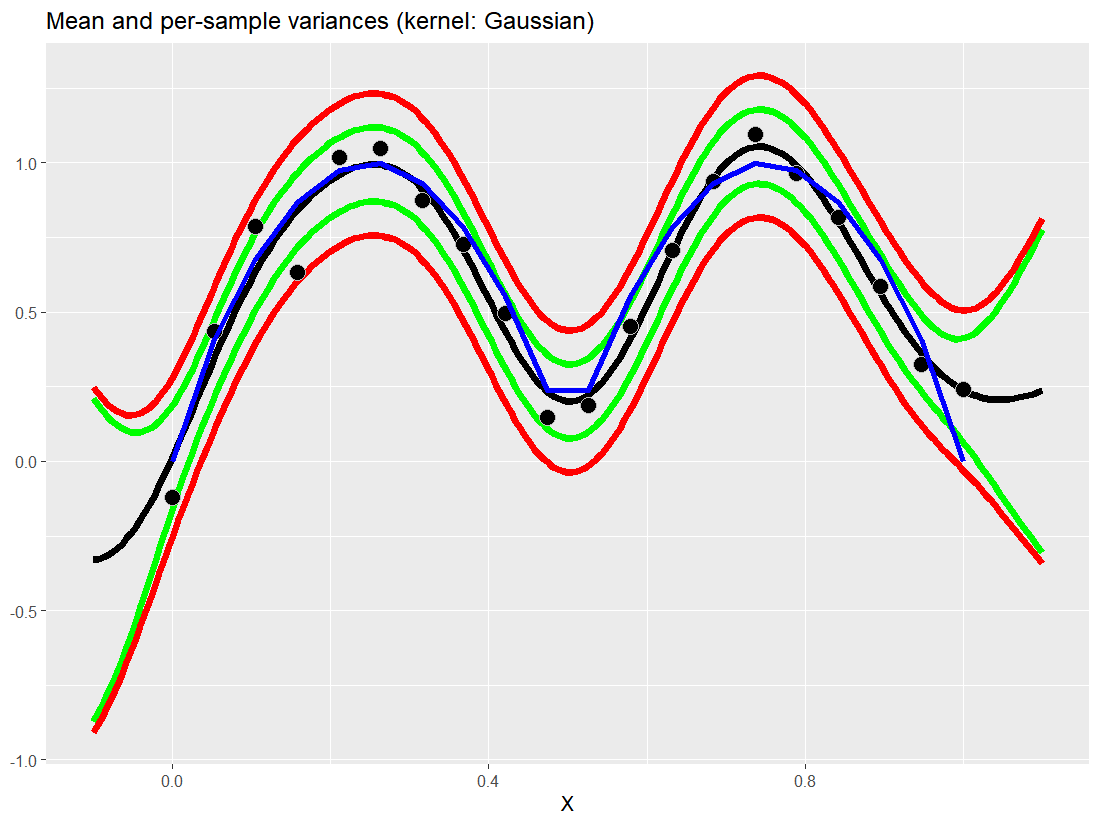
\includegraphics[height=0.5\textwidth]{gaussian_variances.png}
    \caption{
        Plot of a Gaussian process using SE applied to a toy dataset. The toy dataset ($n = 15$) is a data-generating function in blue with some Gaussian noise applied to produce the datapoints in black. The black line represents the expected function from the Gaussian process. The green line represents the 90\% confidence interval around the predictive distribution without the $\sigma^2_n$ term, representing the uncertainty surrounding predictions of the noise-free mean function $f(X)$. The red line represents the 90\% confidence interval with $\sigma^2_n$, representing the uncertainty surrounding predictions of the noisy observations $y$.
    }
\end{figure}

\begin{figure}[h]
    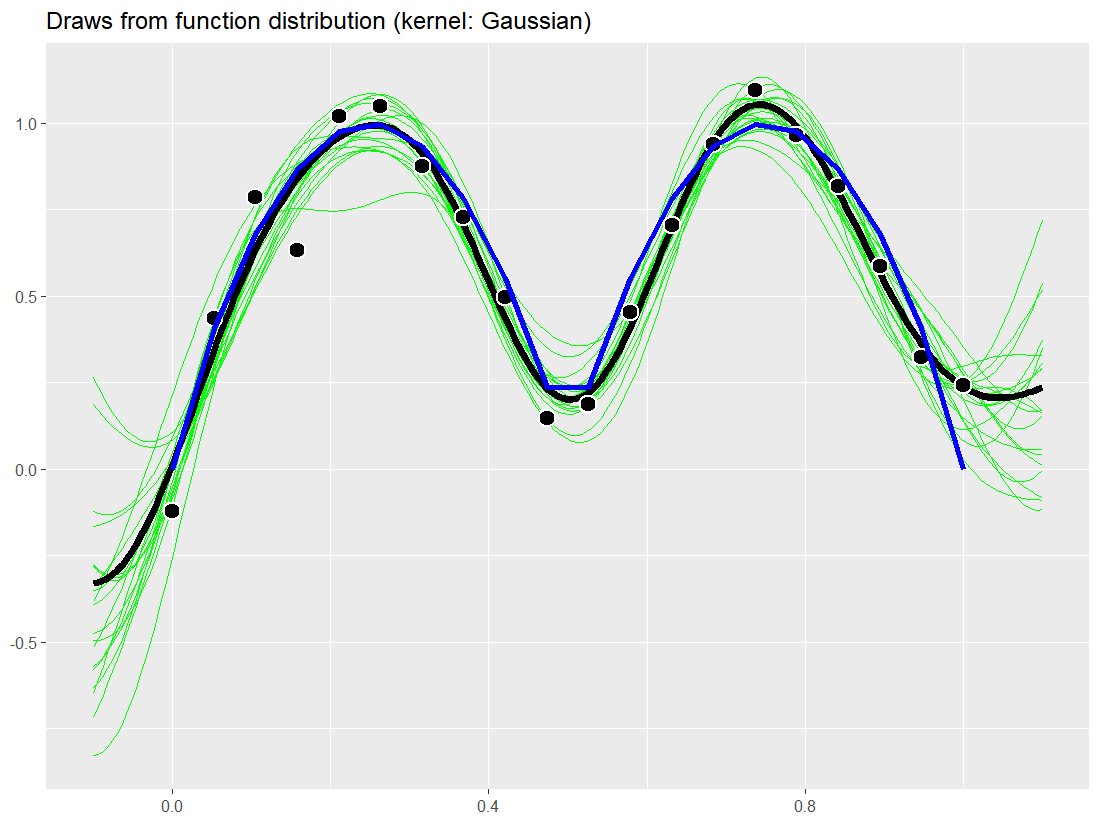
\includegraphics[height=0.5\textwidth]{gaussian_draws.png}
    \caption{
        Plots of functions from a Gaussian process using SE applied to the same toy dataset. The blue line and black datapoints and lines are as before, but the green lines here are a sample of functions drawn from the Gaussian process.
    }
\end{figure}

TODO proof of infinite basis functions, background needed


% Often causes issues since it assumes infinite differentiability. Experts don’t recommend using it. \cite{gaopro}

% TODO fix formatting here
\newpage
\subsubsection{Matern-class}
The Matern class of covariance functions is given by:
\begin{equation*}
    k(X,X') = \frac{2^{1 - \nu}}{\Gamma(\nu)}\left(\frac{\sqrt{2\nu}|X - X'|}{l}\right)^{\nu}K_{\nu}\left(\frac{\sqrt{2\nu}|X - X'|}{l}\right)
\end{equation*}

$l$ is our familiar length scale hyperparameter, but $\nu$ controls how differentiable the function is. 

TODO Bessel function $K_{\nu}$, background needed
Therefore, a a Gaussian process using a Matern class kernel is $k$-times MS differentiable if and only if $\nu > k$. 

We can simplify this by using half-integers, i.e. $\nu = p + 1/2$ where $p$ is a non-negative integer. In this case, the covariance function becomes a product of a polynomial and an exponential:

\begin{equation*}
    k_{\nu = p + 1/2}(X,X') = \exp \left(- \frac{\sqrt{2\nu}|X - X'|}{l} \right) \frac{\Gamma(p+1)}{\Gamma(2p+1)} \sum_{i=0}^p \frac{(p + i)!}{i!(p-i)!} \left( \frac{\sqrt{8\nu r}}{l} \right)^{p-i}
\end{equation*}

$\nu = 1/2$ is equivelant to the exponential covariance function.

TODO formula

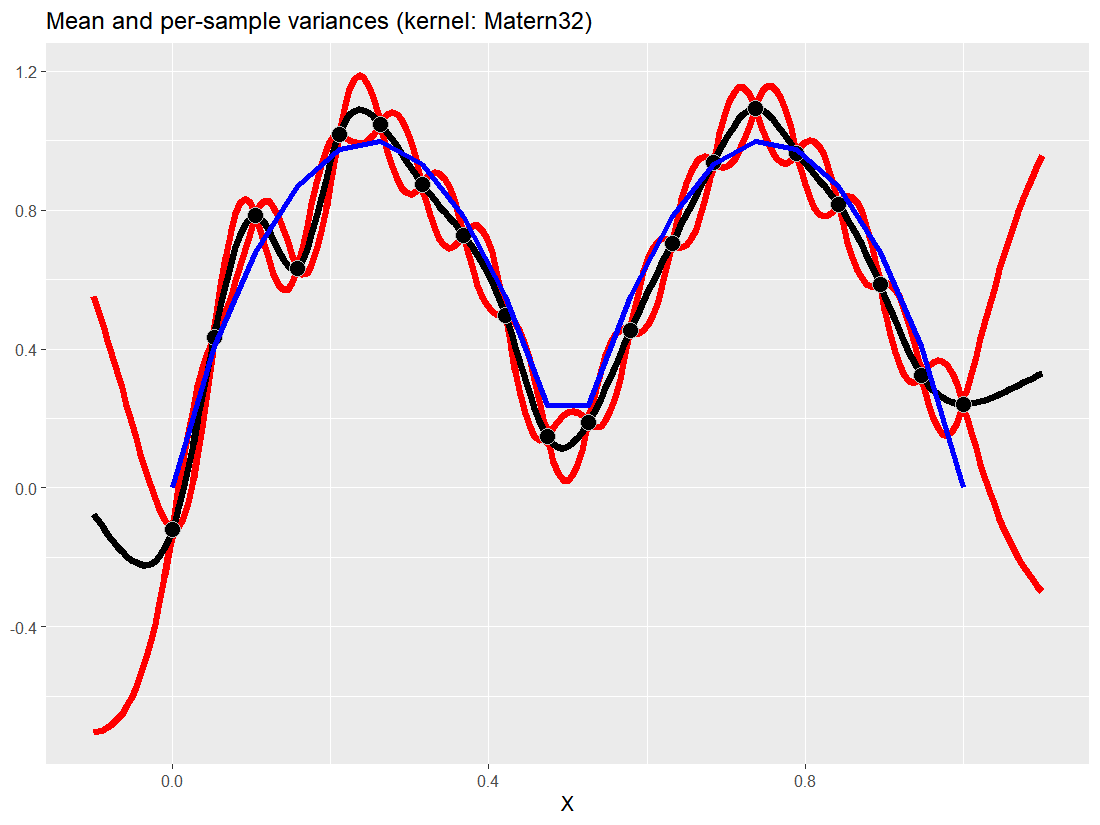
\includegraphics[height=0.5\textwidth]{matern32_variances.png} \\
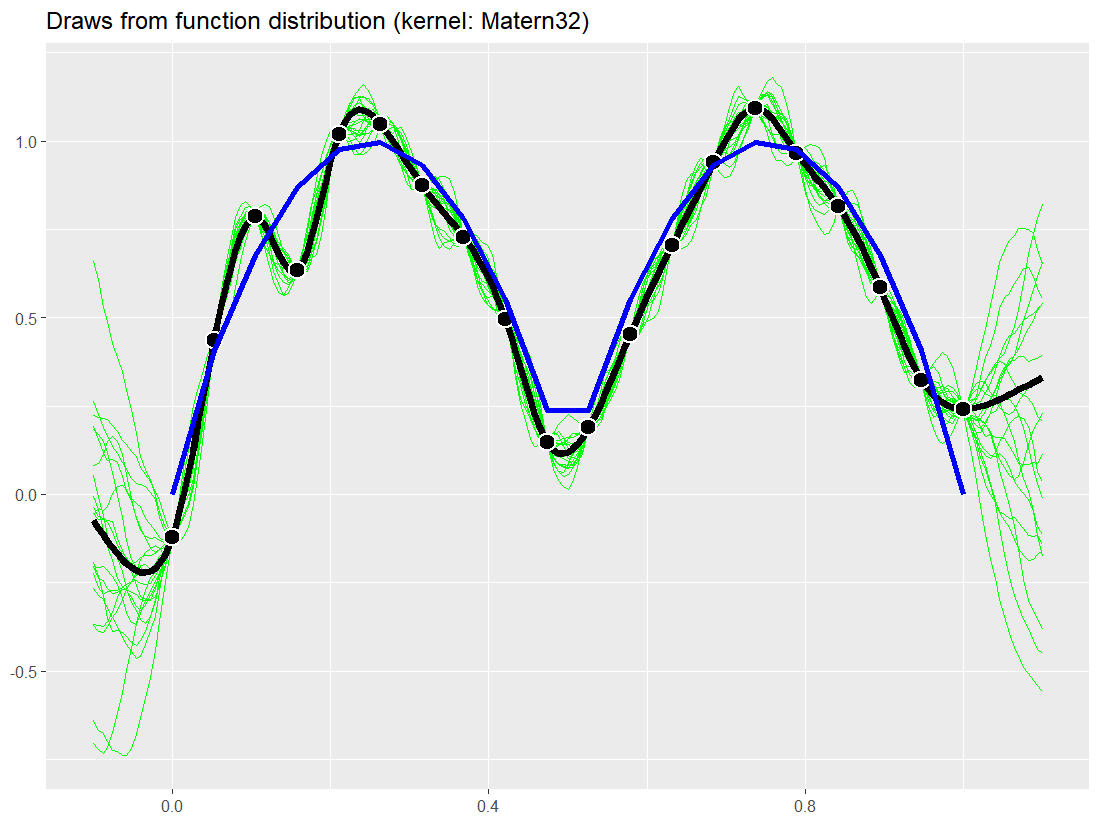
\includegraphics[height=0.5\textwidth]{matern32_draws.png} \\

% Matern 3/2: Assumes one time differentiability. This is often too low of an assumption. \cite{gaopro}

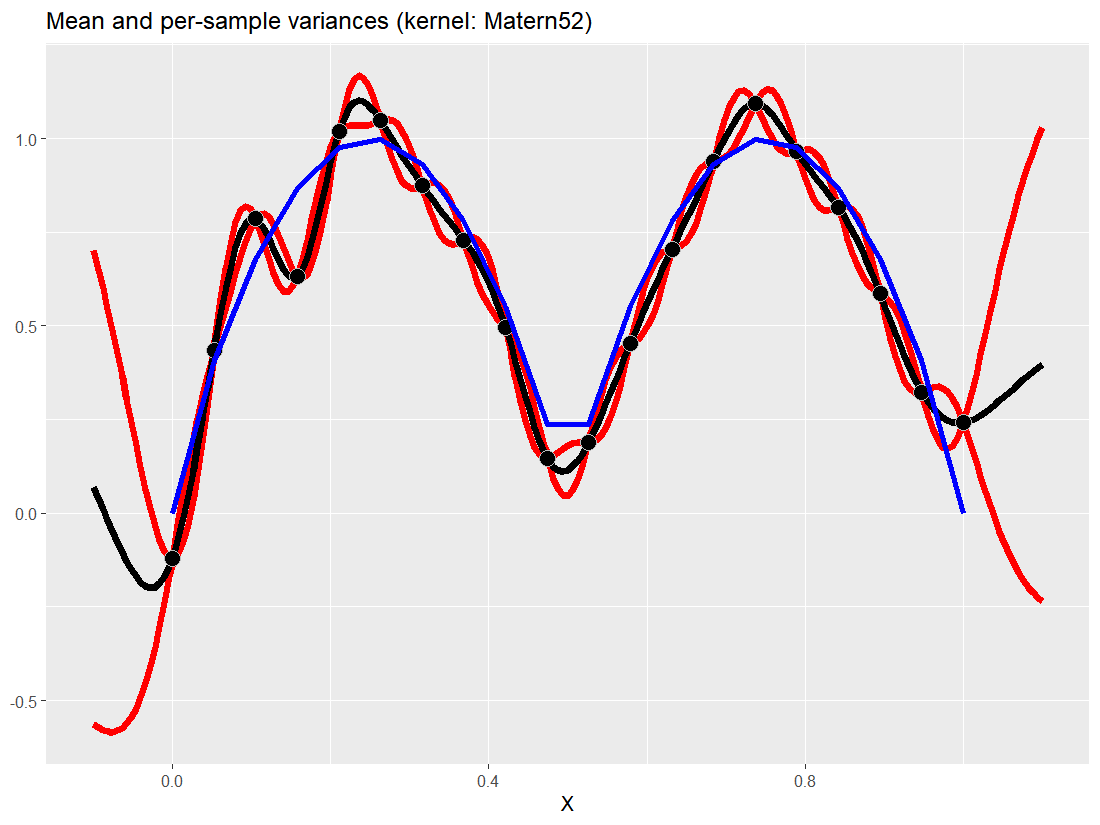
\includegraphics[height=0.5\textwidth]{matern52_variances.png} \\
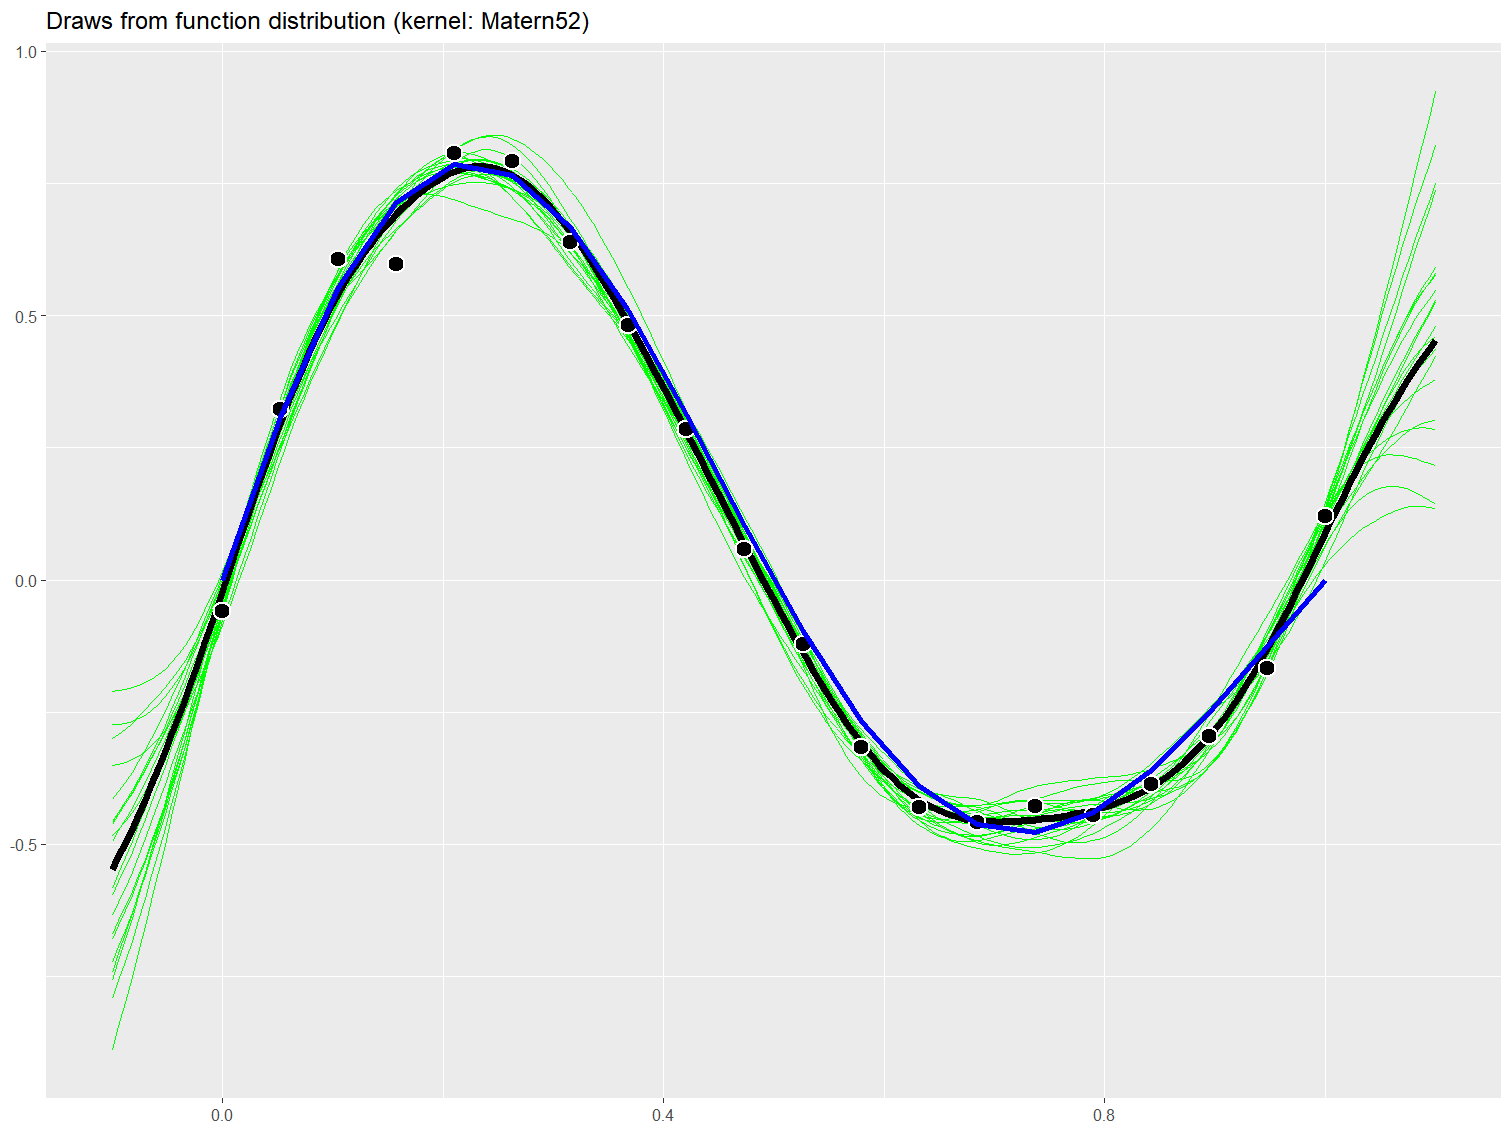
\includegraphics[height=0.5\textwidth]{matern52_draws.png} \\

% Matern 5/2: Assumes two time differentiability. Generally the best. \cite{gaopro}

\subsubsection{Exponential and $\gamma$-exponential}
TODO formulas 

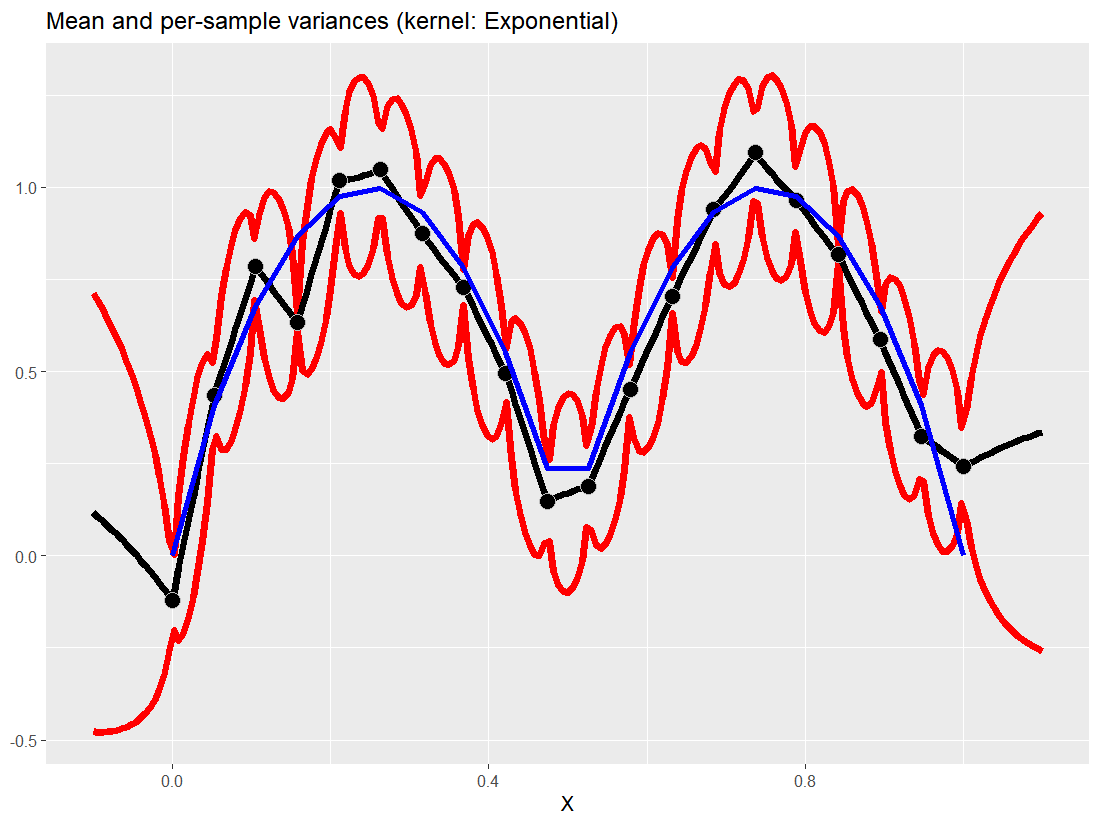
\includegraphics[height=0.5\textwidth]{exp_variances.png} \\
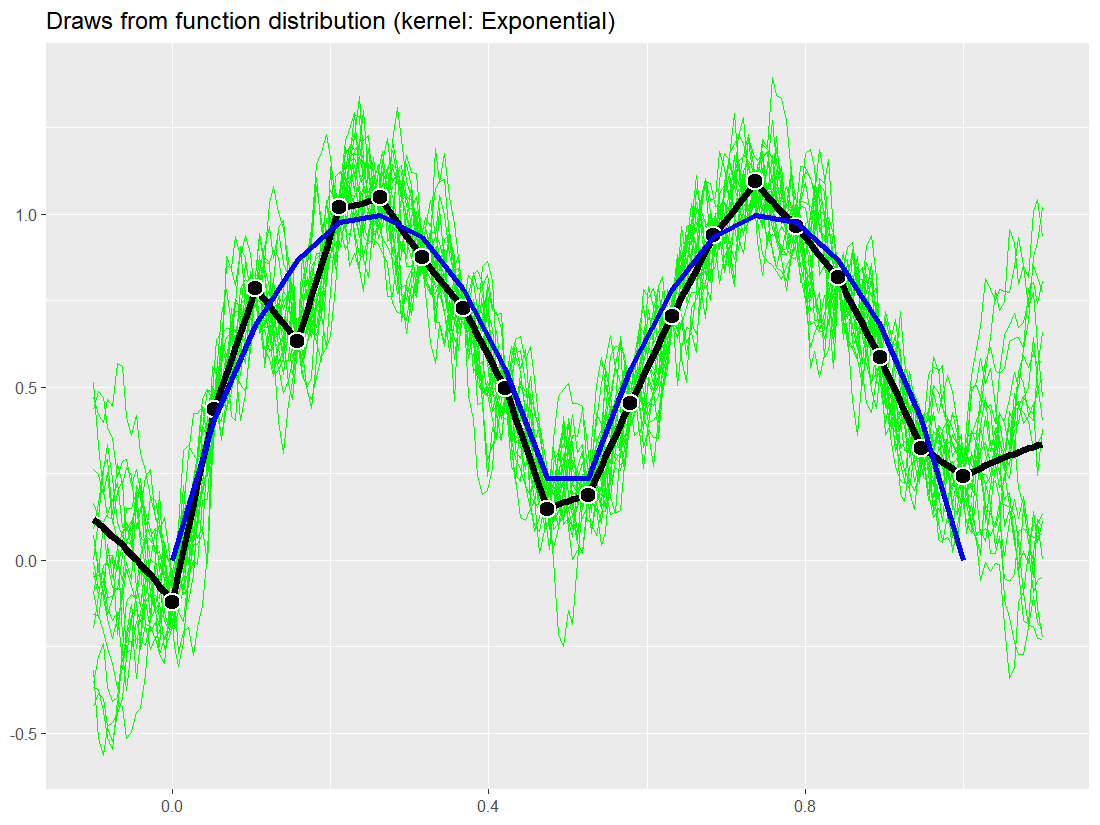
\includegraphics[height=0.5\textwidth]{exp_draws.png} \\
% Exponential: Equivalent to Matern 1/2. Assumes no differentiability. \cite{gaopro}

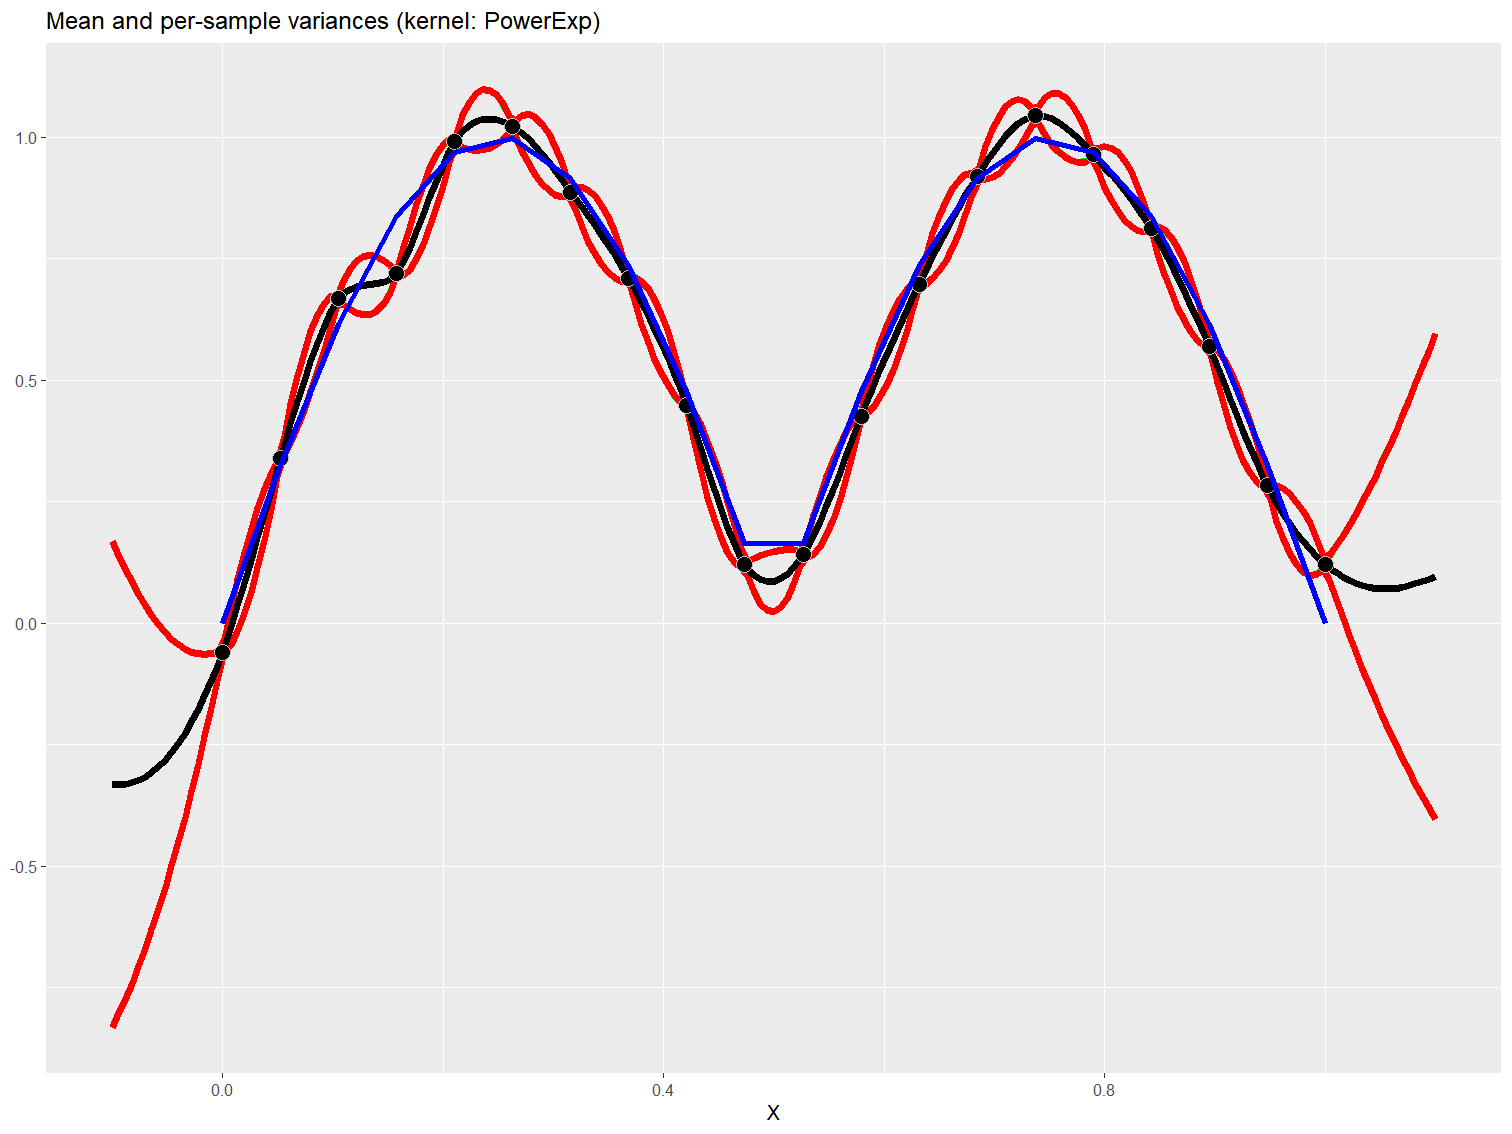
\includegraphics[height=0.5\textwidth]{powerexp_variances.png} \\
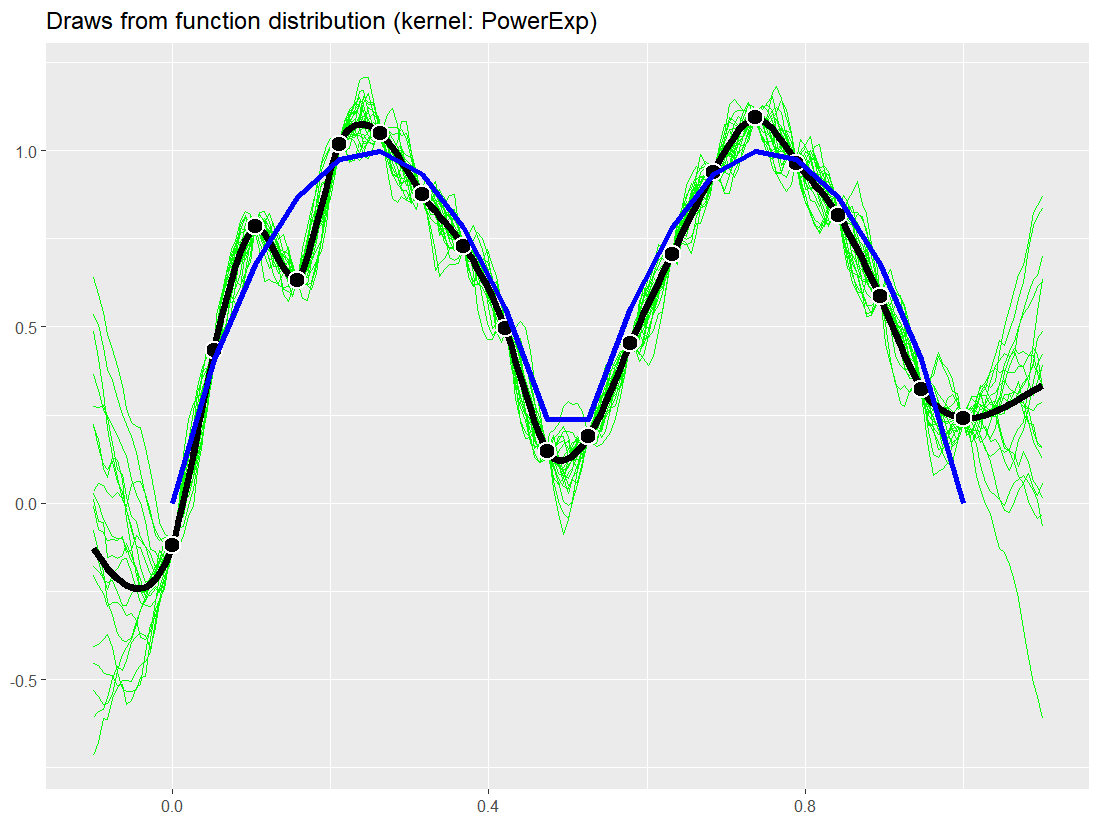
\includegraphics[height=0.5\textwidth]{powerexp_draws.png} \\

\subsubsection{Rational quadratic}
The rational quadratic can be seen as an infinite sum of SE with different length-scales.

TODO formulas

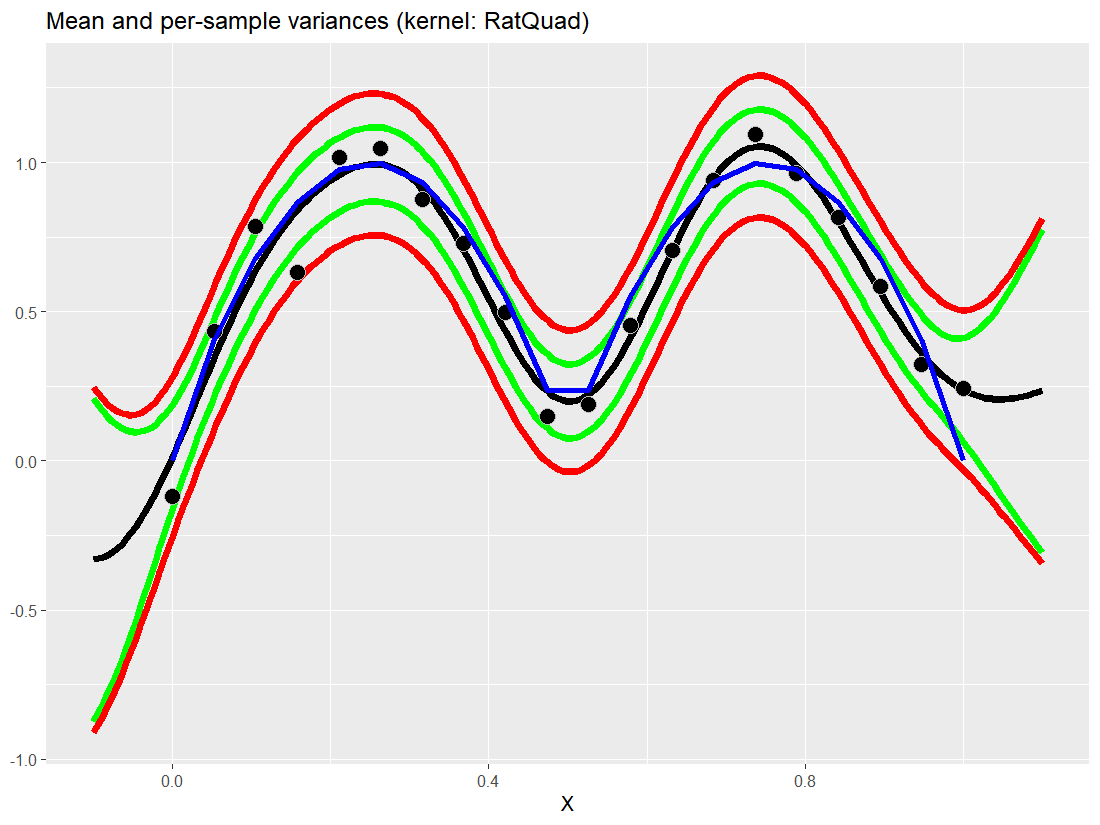
\includegraphics[height=0.5\textwidth]{ratquad_variances.png} \\
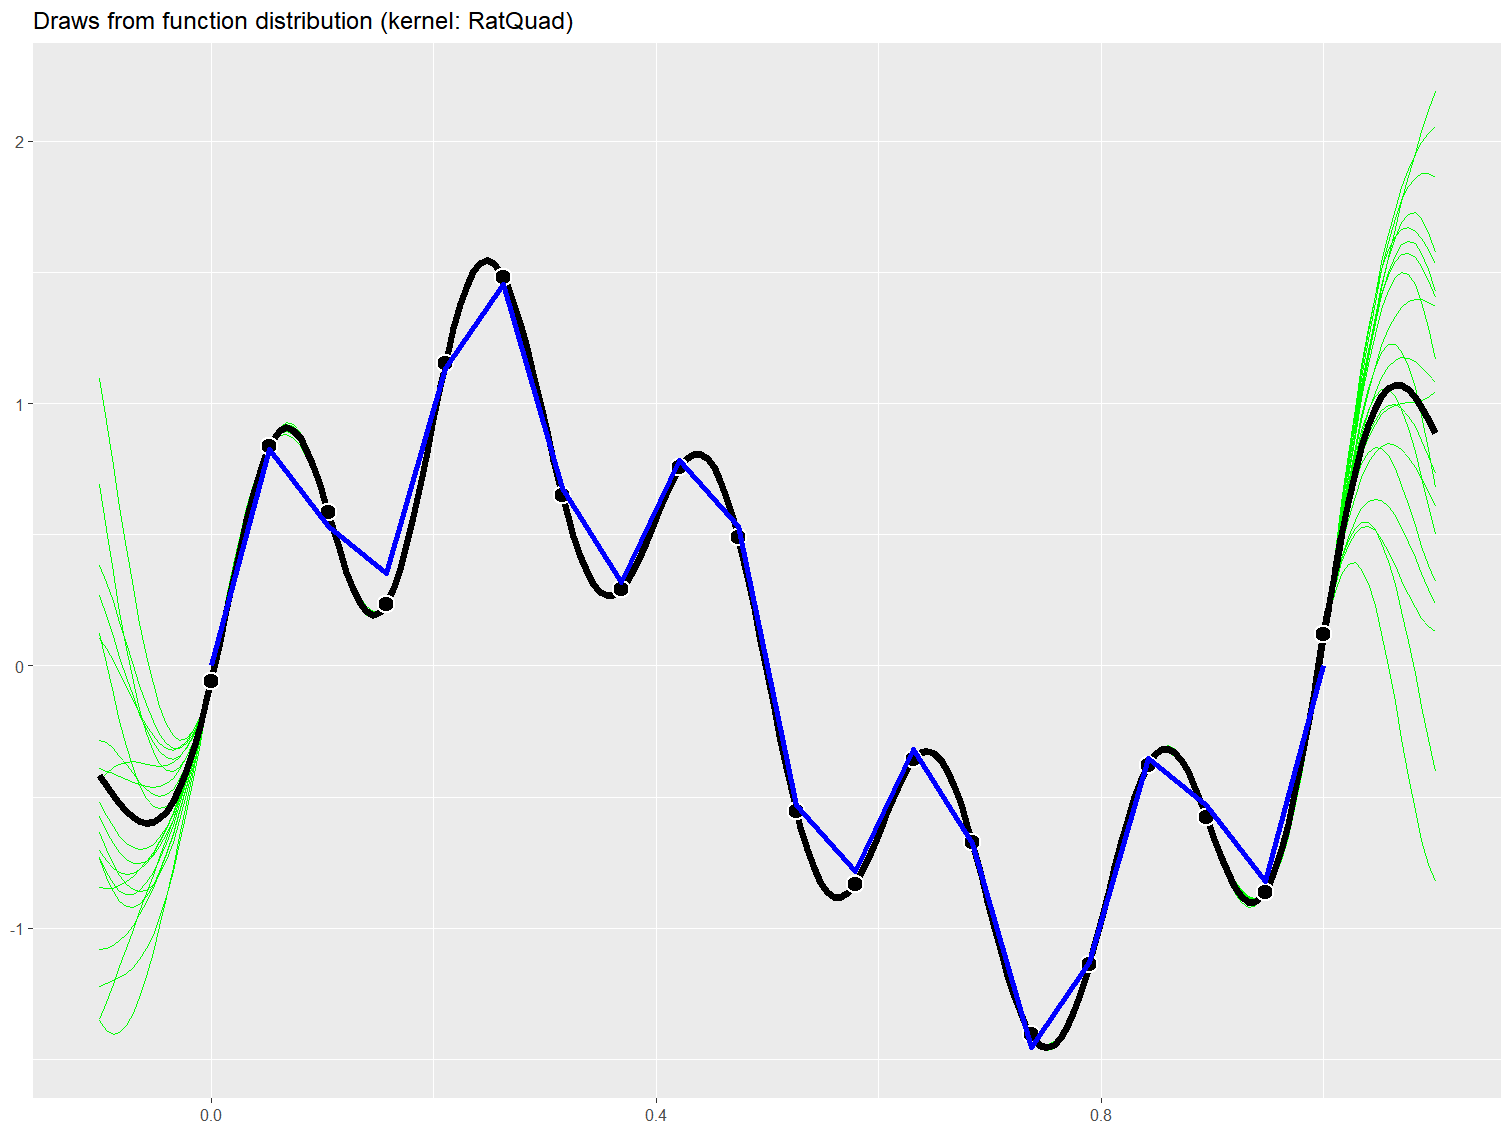
\includegraphics[height=0.5\textwidth]{ratquad_draws.png} \\


\subsection{Non-stationary covariance functions \cite{gp-ml}}

\subsubsection{Sum and product}

\subsubsection{Neural network}

\subsubsection{Warping and periodicity}


\subsection{Language-processing covariance functions \cite{gp-ml}}

\subsubsection{String}

\subsubsection{Fisher}


\subsection{Factor-processing covariance functions \cite{gaopro}}

\subsubsection{Ordered factor}

\subsubsection{Factor}

\subsubsection{Gower factor}

\subsubsection{Indices-ignoring}


\subsection{Deriving kernels \cite{deriving-kernels}}


\subsection{Learning best kernel from data \cite{choosing-kernels}}


\subsection{Additive covariance kernels for high-dimensional learning \cite{additive-kernels}}


\subsection{Hierarchical Bayesian covariance function for hierarchical modelling \cite{hierarchical-kernels}}


\subsection{Free-form covariance matrix for multi-task learning \cite{freeform-kernels}}


\subsection{Combining different kernels for multi-task learning \cite{multi-kernels}}



% \section{Extensions of the Gaussian Process}
% 
% 
% \subsection{Gaussian process regression networks \cite{gprn}}
% 
% 
% \subsection{Variational Gaussian process \cite{vgp}}



\section{Computational Issues}


\subsection{Matrix inversion \cite{big-data}}
Inverting the $[K(X,X) + \sigma^2_nI]$ matrix in our predictive distribution scales poorly with the number of training data points $n$, as inverting the $n \times n$ matrix $X$ that represents our training data is $O(n^3)$. Strategies to approximate the result of this inversion fall into two categories: those that produce a single approximation for the entire dataset, or those that produce several approximations that are "experts" in a particular region of the dataset and combine these local approximations to form a global approximation.

\subsubsection{Global approximations}

\paragraph{Subset-of-data}
The simplest strategy is to use a subset $M$ of $X$ to reduce the cost of inversion to $O(m^3)$, where $m$ is the number of training points in $M$. Although this approach does not address the issues of matrix inversion directly,a theoretical graphon analysis proves that choosing $M$ randomly gives an accuracy of $O(log^{-1/4}m)$ for the predictive mean and variance, which produces more accurate predictions with faster runtimes than sparse approximations as $n$ increases. \cite{random-subsampling} Subset-of-data also requires no analytic assumptions about the kernel.

% using a subset of $M$ that is representative of the entire dataset by clustering the data, e.g. using a k-means algorithm, and using these cluster centroids as our subset. 

We can reduce $m$ needed to achieve the same level of accuracy with a "greedy" approach by determining the gain in likelihood from including each data point $x_i$ in X, adding the maximum gain in likelihood point to $M$ and repeating until the size of $M$ reaches $m$. However, computational savings from reducing $m$ are smaller than the cost of searching $X$ for these centroids $O(n^2m)$. Instead, we can use a "matching pursuit" approach - maintain a cache of the already precomputed kernel values, and use these to compute the gain in likelihood for each point in $X$ in $O(nm^2)$ time. \cite{matching-pursuit}

\paragraph{Sparse kernels}
A sparse kernel is a particularly designed kernel that imposes $k(X,X') = 0$ if $|X - X'|$ is larger than some threshold $d$ to create a sparse covariance matrix. This reduces the number of calculations that need to be performed and computational complexity to $O(an^3)$, where $a$ is the proportion of non-zero entries remaining, but the kernel needs to be carefully designed to work with zeroes and ensure all entries are positive definite to satisfy completeness. TODO sparse RBF

\paragraph{Sparse approximations}
TODO, missing background

\subparagraph{Prior approximation}
\subparagraph{Posterior approximation}
\subparagraph{Structured sparse approximation}


\subsubsection{Local approximations}
TODO

\paragraph{Naive-local-experts}

\paragraph{Mixture-of-experts}

\paragraph{Product-of-experts}


\subsubsection{Improvements}
TODO

\paragraph{Scalability}

\paragraph{Capability}


\subsubsection{Extensions}

\paragraph{Scalable manifold GP}

\paragraph{Scalable deep GP}

\paragraph{Scalable online GP}

\paragraph{Scalable multi-task GP}

\paragraph{Scalable recurrent GP}

\paragraph{Scalable GP classification}



\section{Applying a Gaussian process to TBD}
Possible domains:


\subsection{Materials science \cite{materials}}


\subsection{Cosmography \cite{cosmography}}


\subsection{Statistical emulators \cite{emulators}}


\subsection{Signals processing \cite{signals-processing}}



\section{Conclusion}




\printbibliography

\end{document}
